\chapter{Projets annexes scientifique hors académique}
\label{annexe_projets_annexe}

\section{Bioinfo-fr.net}

Le doctorat est l'occasion d'acquérir et par la suite de partager de nombreuses connaissances. Co-administratrice et auteur sur le blog \href{https://bioinfo-fr.net/}{bioinfo-fr.net}, ce blog vise à partager des tutoriels sur des analyses, à répondre à des questions communément posées aux bio-informaticiens, et à faire profiter la communauté francophone d'astuces amenées par tous. Ce blog communautaire est également l'occasion de parler de façon plus légère et décontractée de sujet important tout en restant rigoureux dans les explications. J'ai donc moi-même pu continuer de contribuer à cet effort durant mon doctorat avec les articles suivant qui ont été notamment inspirés par mes travaux :

\begin{itemize}
    \item \href{https://bioinfo-fr.net/packrat-ou-comment-gerer-ses-packages-r-par-projet}{Packrat ou comment gérer ses packages R par projet}, mars 2017
    \item \href{https://bioinfo-fr.net/enquete-bioinfo-fr-2018-portrait-de-bioinfo}{Enquête Bioinfo-fr 2018 : un portrait de la bioinformatique}, juin 2018
    \item \href{https://bioinfo-fr.net/grandes-questions-doctorant-debutant}{Les grandes questions du doctorant en devenir/débutant}, novembre 2018
    \item \href{https://bioinfo-fr.net/la-resistance-aux-antibiotiques-vu-cote-bioinfo}{La bio-informatique au service de l’antibiorésistance}, février 2019
    \item \href{https://bioinfo-fr.net/analyses-bioinformatiques-du-coronavirus-2019-ncov-pourquoi-et-comment}{Analyses bioinformatiques du coronavirus 2019-nCoV : pourquoi et comment ?}, février 2020, co-auteure
    \item \href{https://bioinfo-fr.net/contrarie-par-les-diagrammes-de-venn-decouvrez-les-diagrammes-upset}{Contrarié par les diagrammes de Venn ? Découvrez les diagrammes UpSet}, février 2020
    \item \href{https://bioinfo-fr.net/pourquoi-et-comment-deposer-un-package-r-sur-bioconductor}{Pourquoi et comment déposer un package R sur Bioconductor ?}, juin 2020.
\end{itemize}

\section{Illustration scientifique}

Comme visible dans les figures parcourant cette thèse et mes articles de blog, cette thèse a également été l'occasion de développer ma compétente d'illustration scientifique. À titre d'exemple, voici quelques autres travaux originaux réalisés dans divers contextes scientifiques : 

\begin{figure}[p]
    \centering
    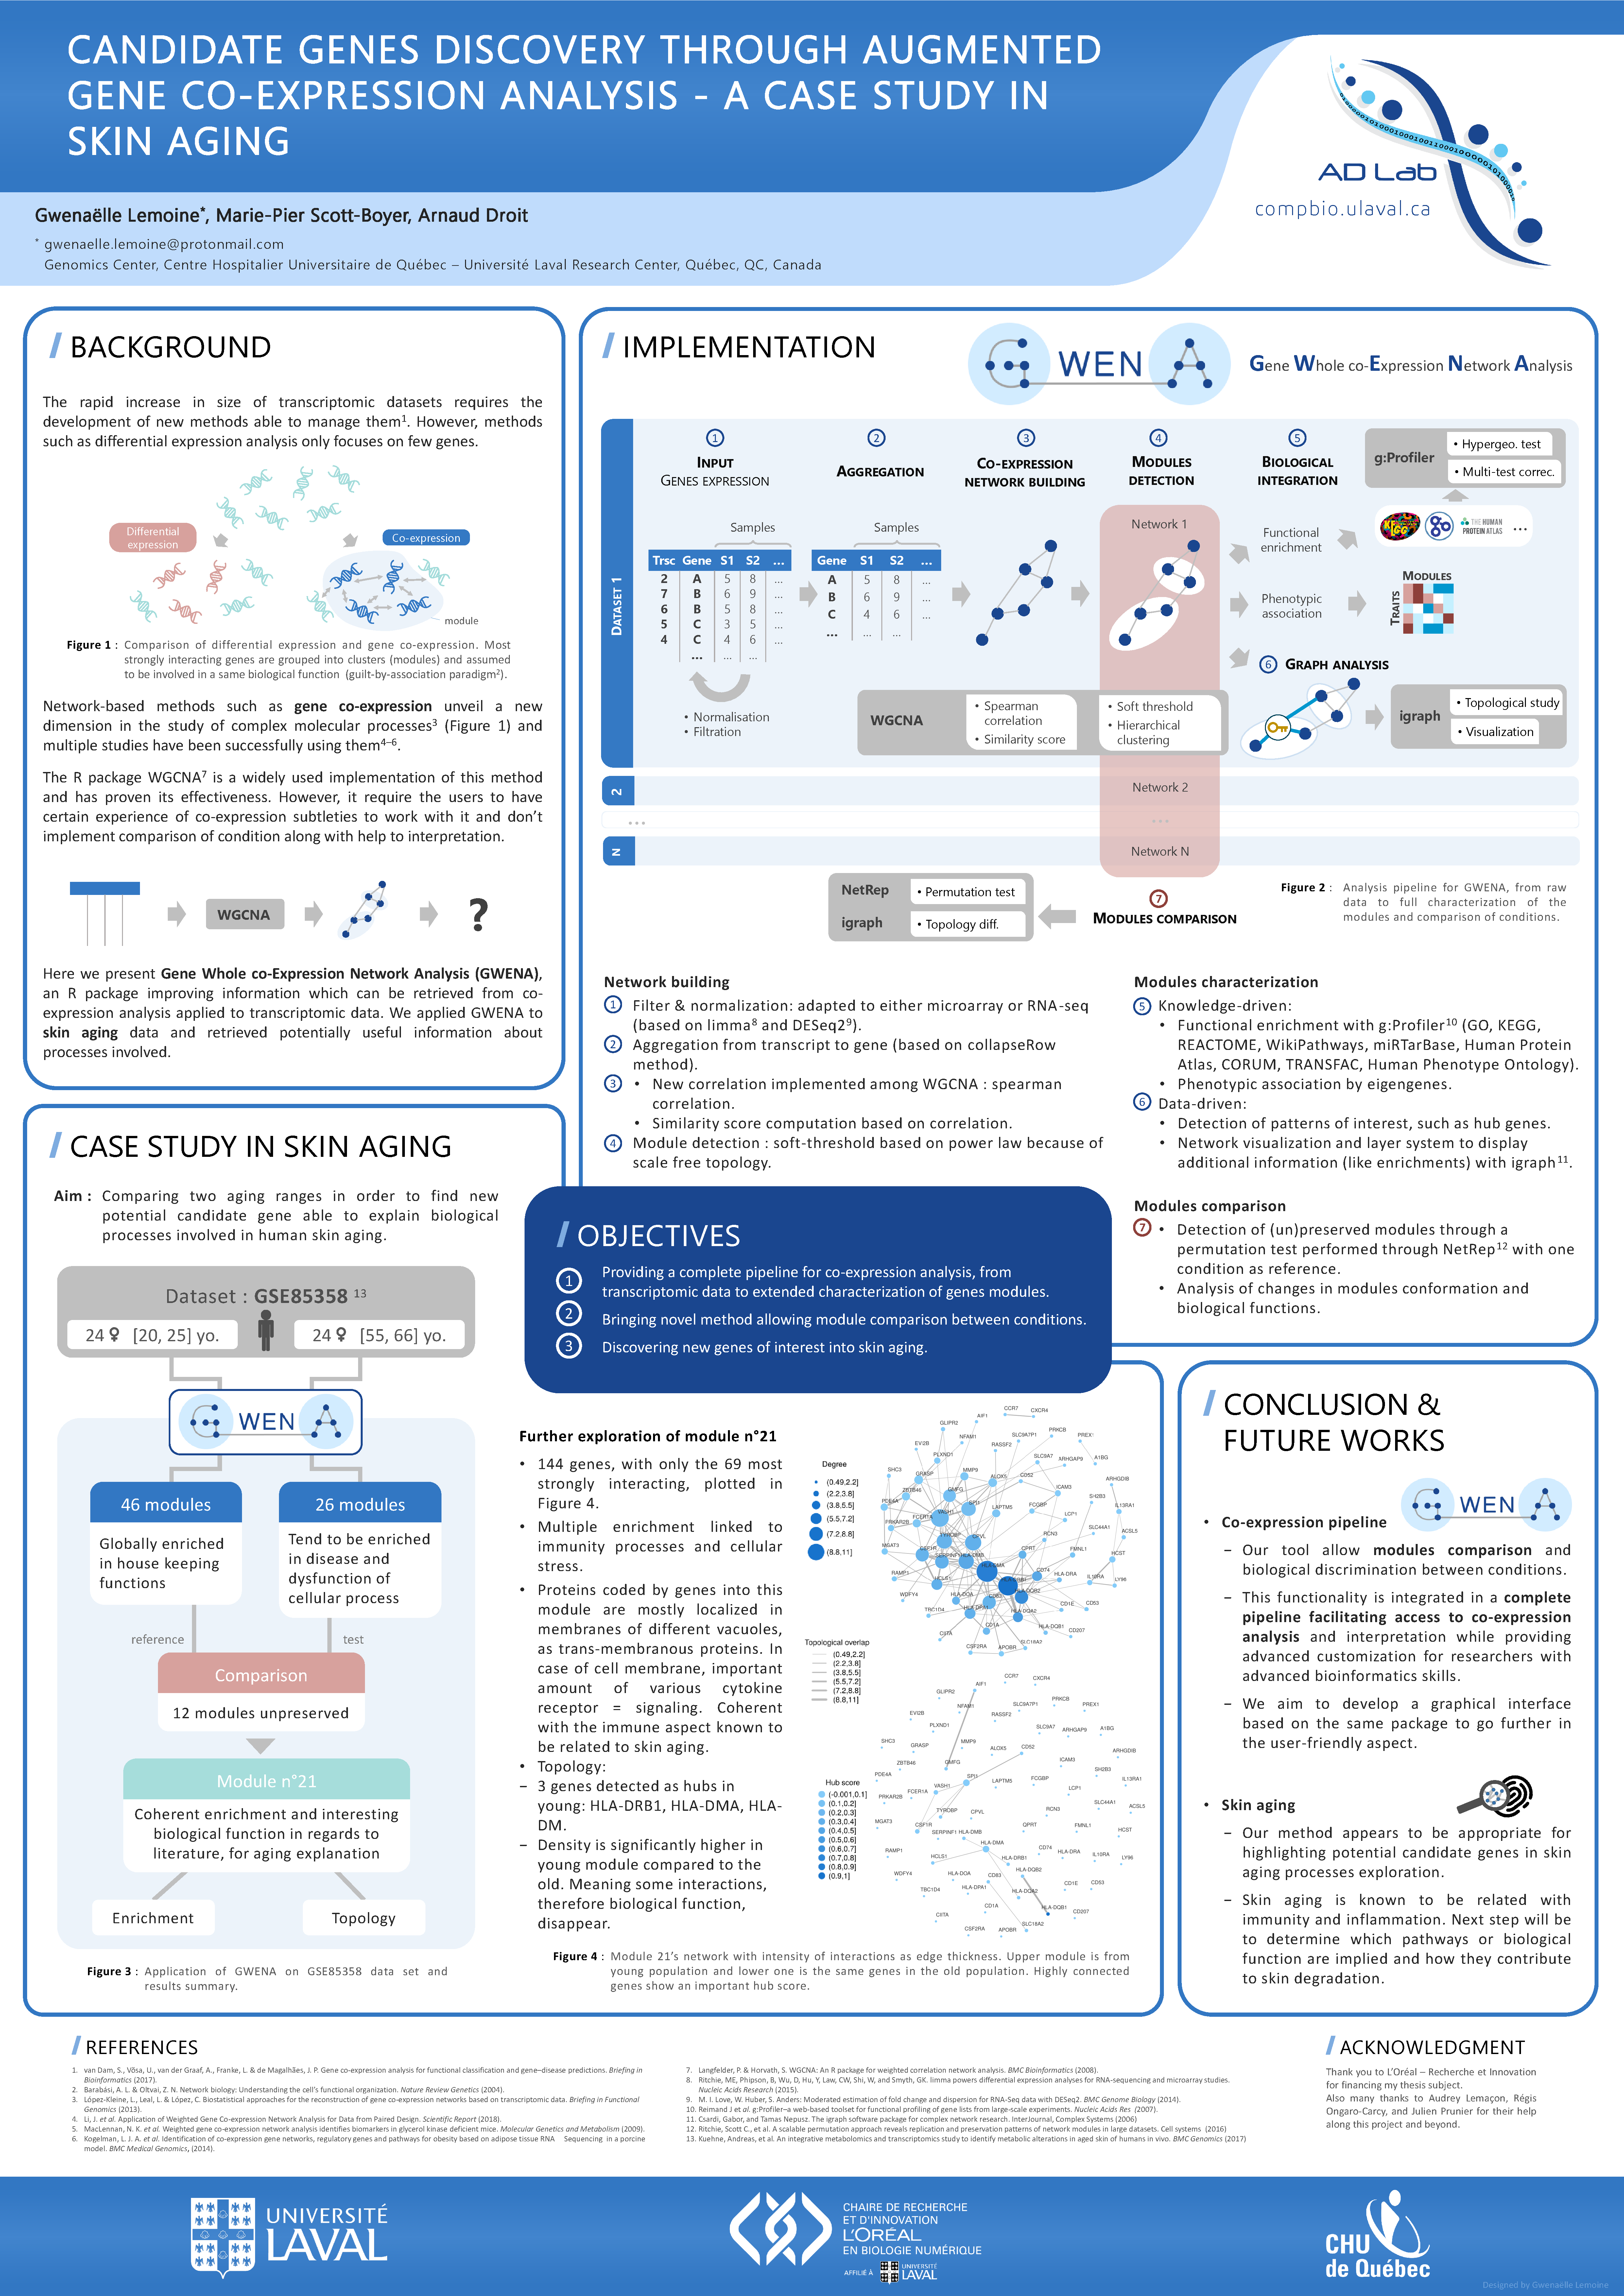
\includegraphics[width=\textwidth]{img/annexe_projets_annexe/20190700_ISCMECCB_ppt.pdf}
    \caption{Affiche présentée à la bi-conférence internationale ISMB/ECCB en 2019}
    \label{fig:annexe_poster_ismb_eccb}
\end{figure}

\begin{figure}
    \centering
    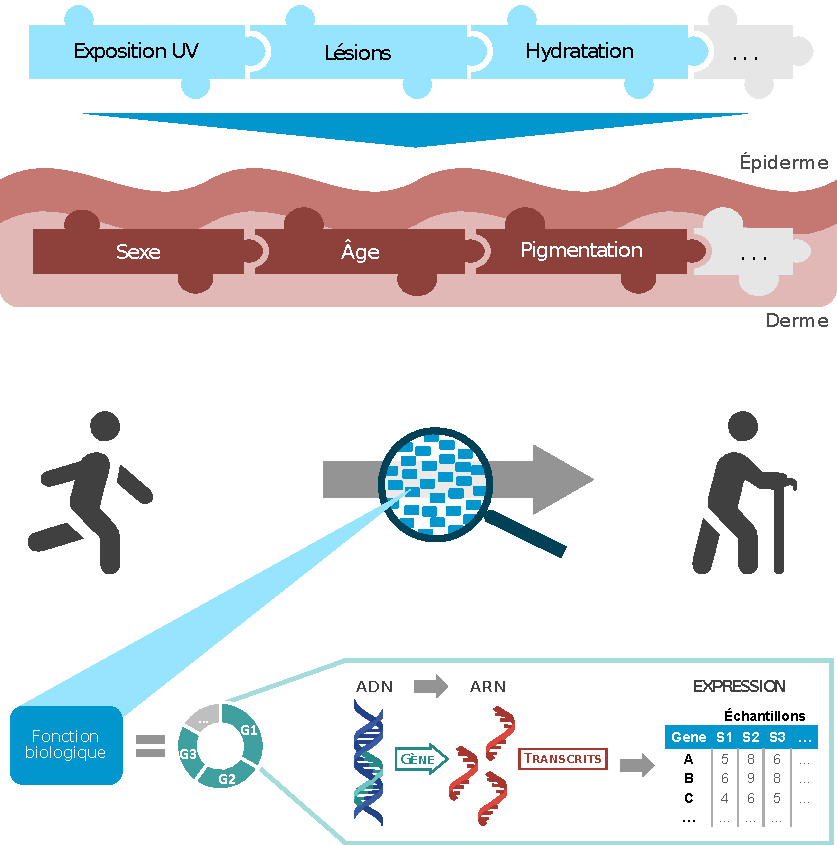
\includegraphics{img/annexe_projets_annexe/20190312_TeaAndLearn_ReuLabo_avancement.pdf}
    \caption{Illustration de la contribution des facteurs intrinsèques et extrinsèques au vieillissement de la peau et leur perception via l'expression des gènes. Réalisé pour une présentation de séminaire étudiant au CHU de Québec-Université Laval.}
    \label{fig:annexe_schema_aging_skin_transcripto}
\end{figure}

\begin{figure}
    \centering
    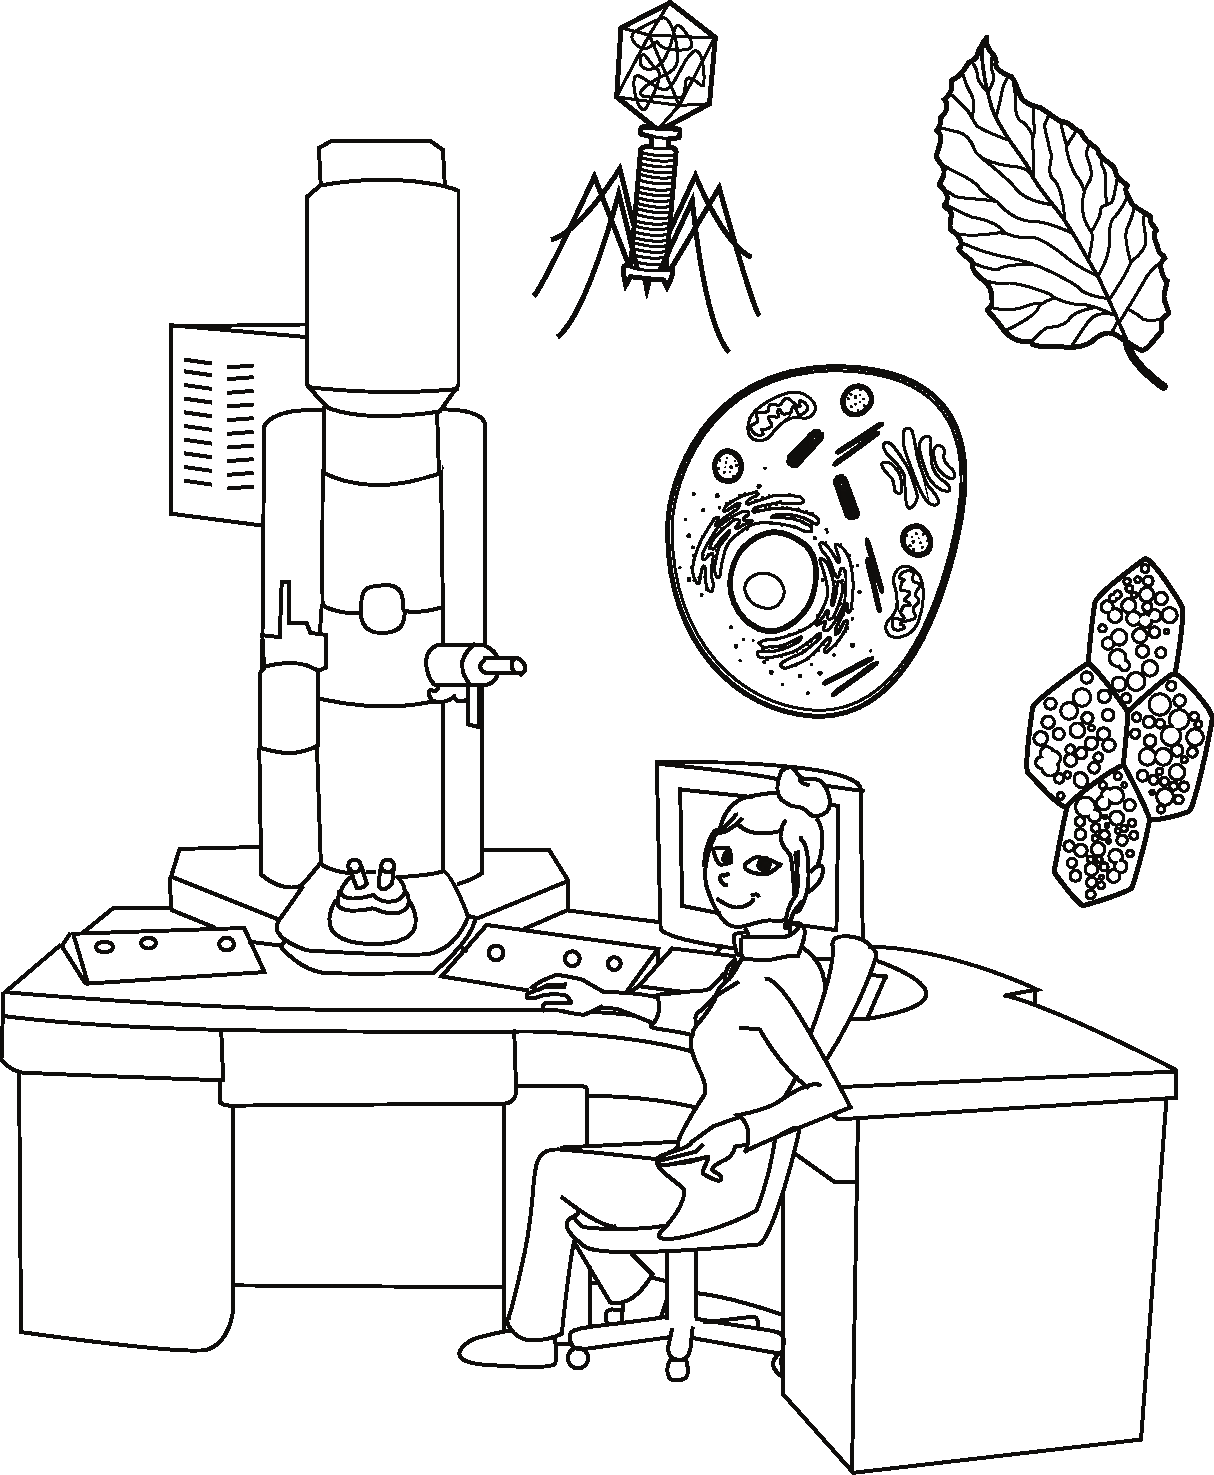
\includegraphics[width=0.8\textwidth]{img/annexe_projets_annexe/these_amandine.pdf}
    \caption{Ensemble d'illustrations réalisées pour la thèse d'Amandine Verguet en microscopie électronique en transmission appliquée à des échantillons biologiques \cite{Verguet2019Dec}}
    \label{fig:annexe_these_amandine}
\end{figure}
